\documentclass[xcolor=table]{beamer}

\graphicspath{{figs/}{./figs/}}
\mode<presentation>
{
%  \usetheme{Warsaw}
  \usetheme{Frankfurt}
%  \setbeamercovered{transparent}
  \usecolortheme{crane}
  \setbeamertemplate{navigation symbols}{}
  \setbeamertemplate{section in toc shaded}[default][60]
  \setbeamertemplate{subsection in toc shaded}[default][50]
  \setbeamertemplate{footline}[frame number]
}


\mode<handout>
{
  \beamertemplatesolidbackgroundcolor{black!5}
  \usecolortheme{dove}
%  \usecolortheme{seagull}
}

\usepackage{url}
\usepackage{ulem}
\usepackage{animate}

% Please add the following required packages to your document preamble:
\usepackage{xcolor}
% If you use beamer only pass "xcolor=table" option, i.e. \documentclass[xcolor=table]{beamer}

\title{Diversity is too important to be left to women}

\author[hmd1]{Hannah Dee \\
  \texttt{hmd1@aber.ac.uk}} 
\date{}
\institute[]{ACCU Keynote, March 2022\\
  Aberystwyth University, Department of Computer Science}



%\beamerdefaultoverlayspecification{<+->}

\AtBeginSection[]
{
  \begin{frame}<beamer>
    \frametitle{Outline}
    \tableofcontents[currentsection,currentsubsection,hideothersubsections]
  \end{frame}
}

\begin{document}

\begin{frame}
  \titlepage
\end{frame}

%%%%%%%%%%%%%%%%%%%%%%%%%%%%%%%%%%%%%%%%%%%%%%%%%%%%%%%%%%%%%%%%%

\section{Intro}

\begin{frame}{What gives me the right to talk about this stuff?}
	\begin{itemize}
		\item Is woman
		\item Is technical
		\item Has read loads of books
		\item On the committee of BCSWomen since 2007
		\item Started the UK's first conference for women undergrads
	\end{itemize}
\end{frame}

\begin{frame}{Karen Sp\"{a}rck Jones} 
	\begin{columns}
		\begin{column}{0.5\textwidth}

	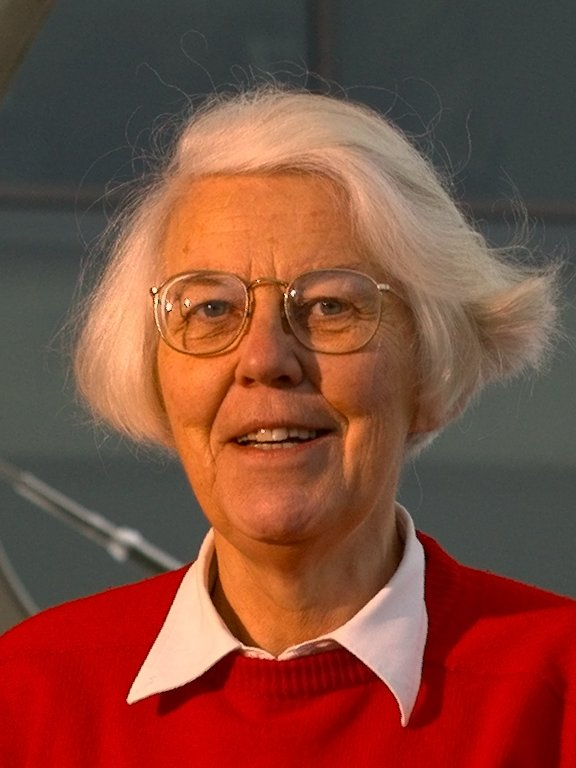
\includegraphics[width=4cm]{ksj.jpg}

	\tiny{University of Cambridge, CC BY 2.5 \url{https://creativecommons.org/licenses/by/2.5}, via Wikimedia Commons}

		\end{column}
		\begin{column}{0.5\textwidth}

		``Computing is too important to be left to men''

			\vspace{0.5em}

			2007
		\end{column}
		\end{columns}
\end{frame}

\begin{frame}{The problem of talking about diversity}

	\begin{columns}
		\begin{column}{0.5\textwidth}
	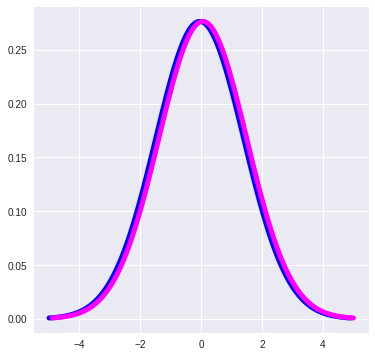
\includegraphics[width=5cm]{gender_diff.png}
		\end{column}
		\begin{column}{0.5\textwidth}
			\sout{Men are from mars, women are from venus} 

			\vspace{0.5em}

			People are from earth
		\end{column}
		\end{columns}
\end{frame}

\begin{frame}{General $\rightarrow$ Specific $\rightarrow$ General}

It is simultaneously possible for there to be \ldots

	\begin{itemize}
		\item very little evidence of gender differences in technical ability
		\item some exceptionally talented guys 
		
		\item some really useless women
	\end{itemize}

	The plural of anecdote isn't data

\end{frame}


\begin{frame}{We've come a long way baby}

	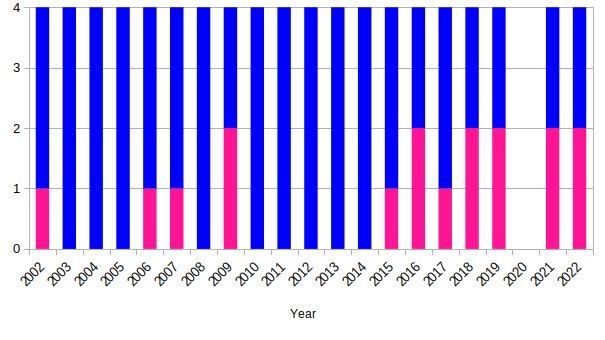
\includegraphics[width=10cm]{accu_key.png}
\end{frame}
\begin{frame}{So isn't diversity in tech a solved problem?}

	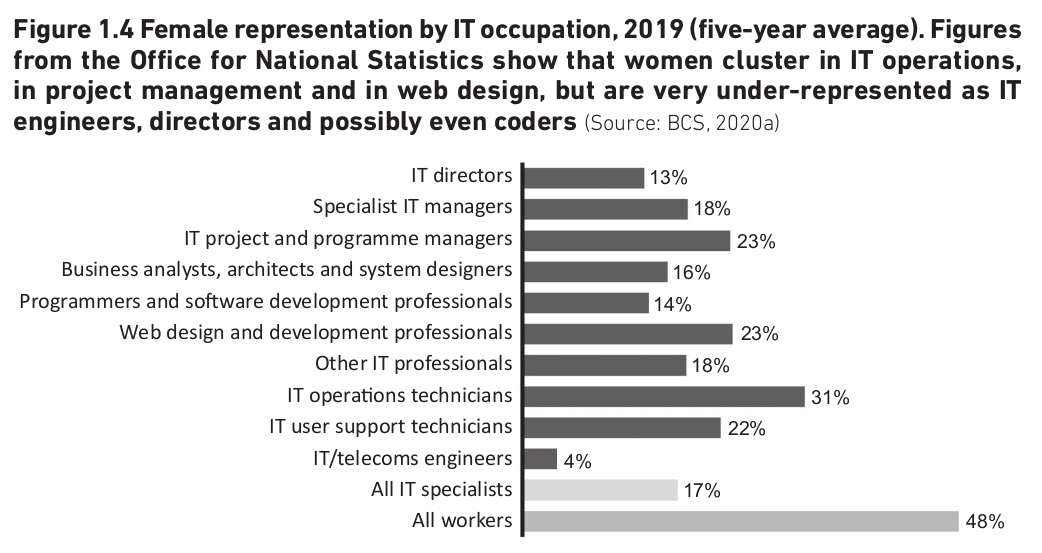
\includegraphics[width=10cm]{it_profession_gender.png}

	\tiny{Source: Women in Tech: A practical guide to increasing gender diversity and inclusion, BCS Publishing \url{https://shop.bcs.org/store/221/detail/workgroup?id=3-221-9781780175614}}
\end{frame}

\begin{frame}{Diversity in tech isn't just gender}

	When there's one clear majority group in a profession, that dominant group's characteristics tend to dominate the profession.  Sociologists talk about``\textbf{Gender role spillover}'' or ``sex role spillover'' when analysing professions with major gender imbalances


	\vspace{0.5em}

	Gender is one of the easier characteristics to measure.  	

	\vspace{0.5em}

	With other characteristics (age, disability, gender reassignment, marriage and civil partnership, pregnancy and maternity, race, religion or belief, sex, sexual orientation) it's harder to point to a norm, but we need to think about these and also about \textbf{intersectionality}.

\end{frame}
\section{Why}

\subsection{It's bad for business}

\begin{frame}{McKinsey etc. }

\end{frame}
\begin{frame}{Diverse boards}

	Financial Reporting council (FRC), 2021, FT350:

More gender diversity generally means 
	\begin{itemize}
		\item better financial performance
		\item less shareholder dissent
		\item more decentralisation in operational practices
		\item more consensus
		\item less overconfidence
	\end{itemize}


	\tiny{\url{https://www.frc.org.uk/getattachment/3cc05eae-2024-45d8-b14c-abb2ac7497aa/FRC-Board-Diversity-and-Effectiveness-in-FTSE-350-Companies.pdf}}
\end{frame}

\begin{frame}{Business motivation}
	\begin{columns}
		\begin{column}{0.5\textwidth}
	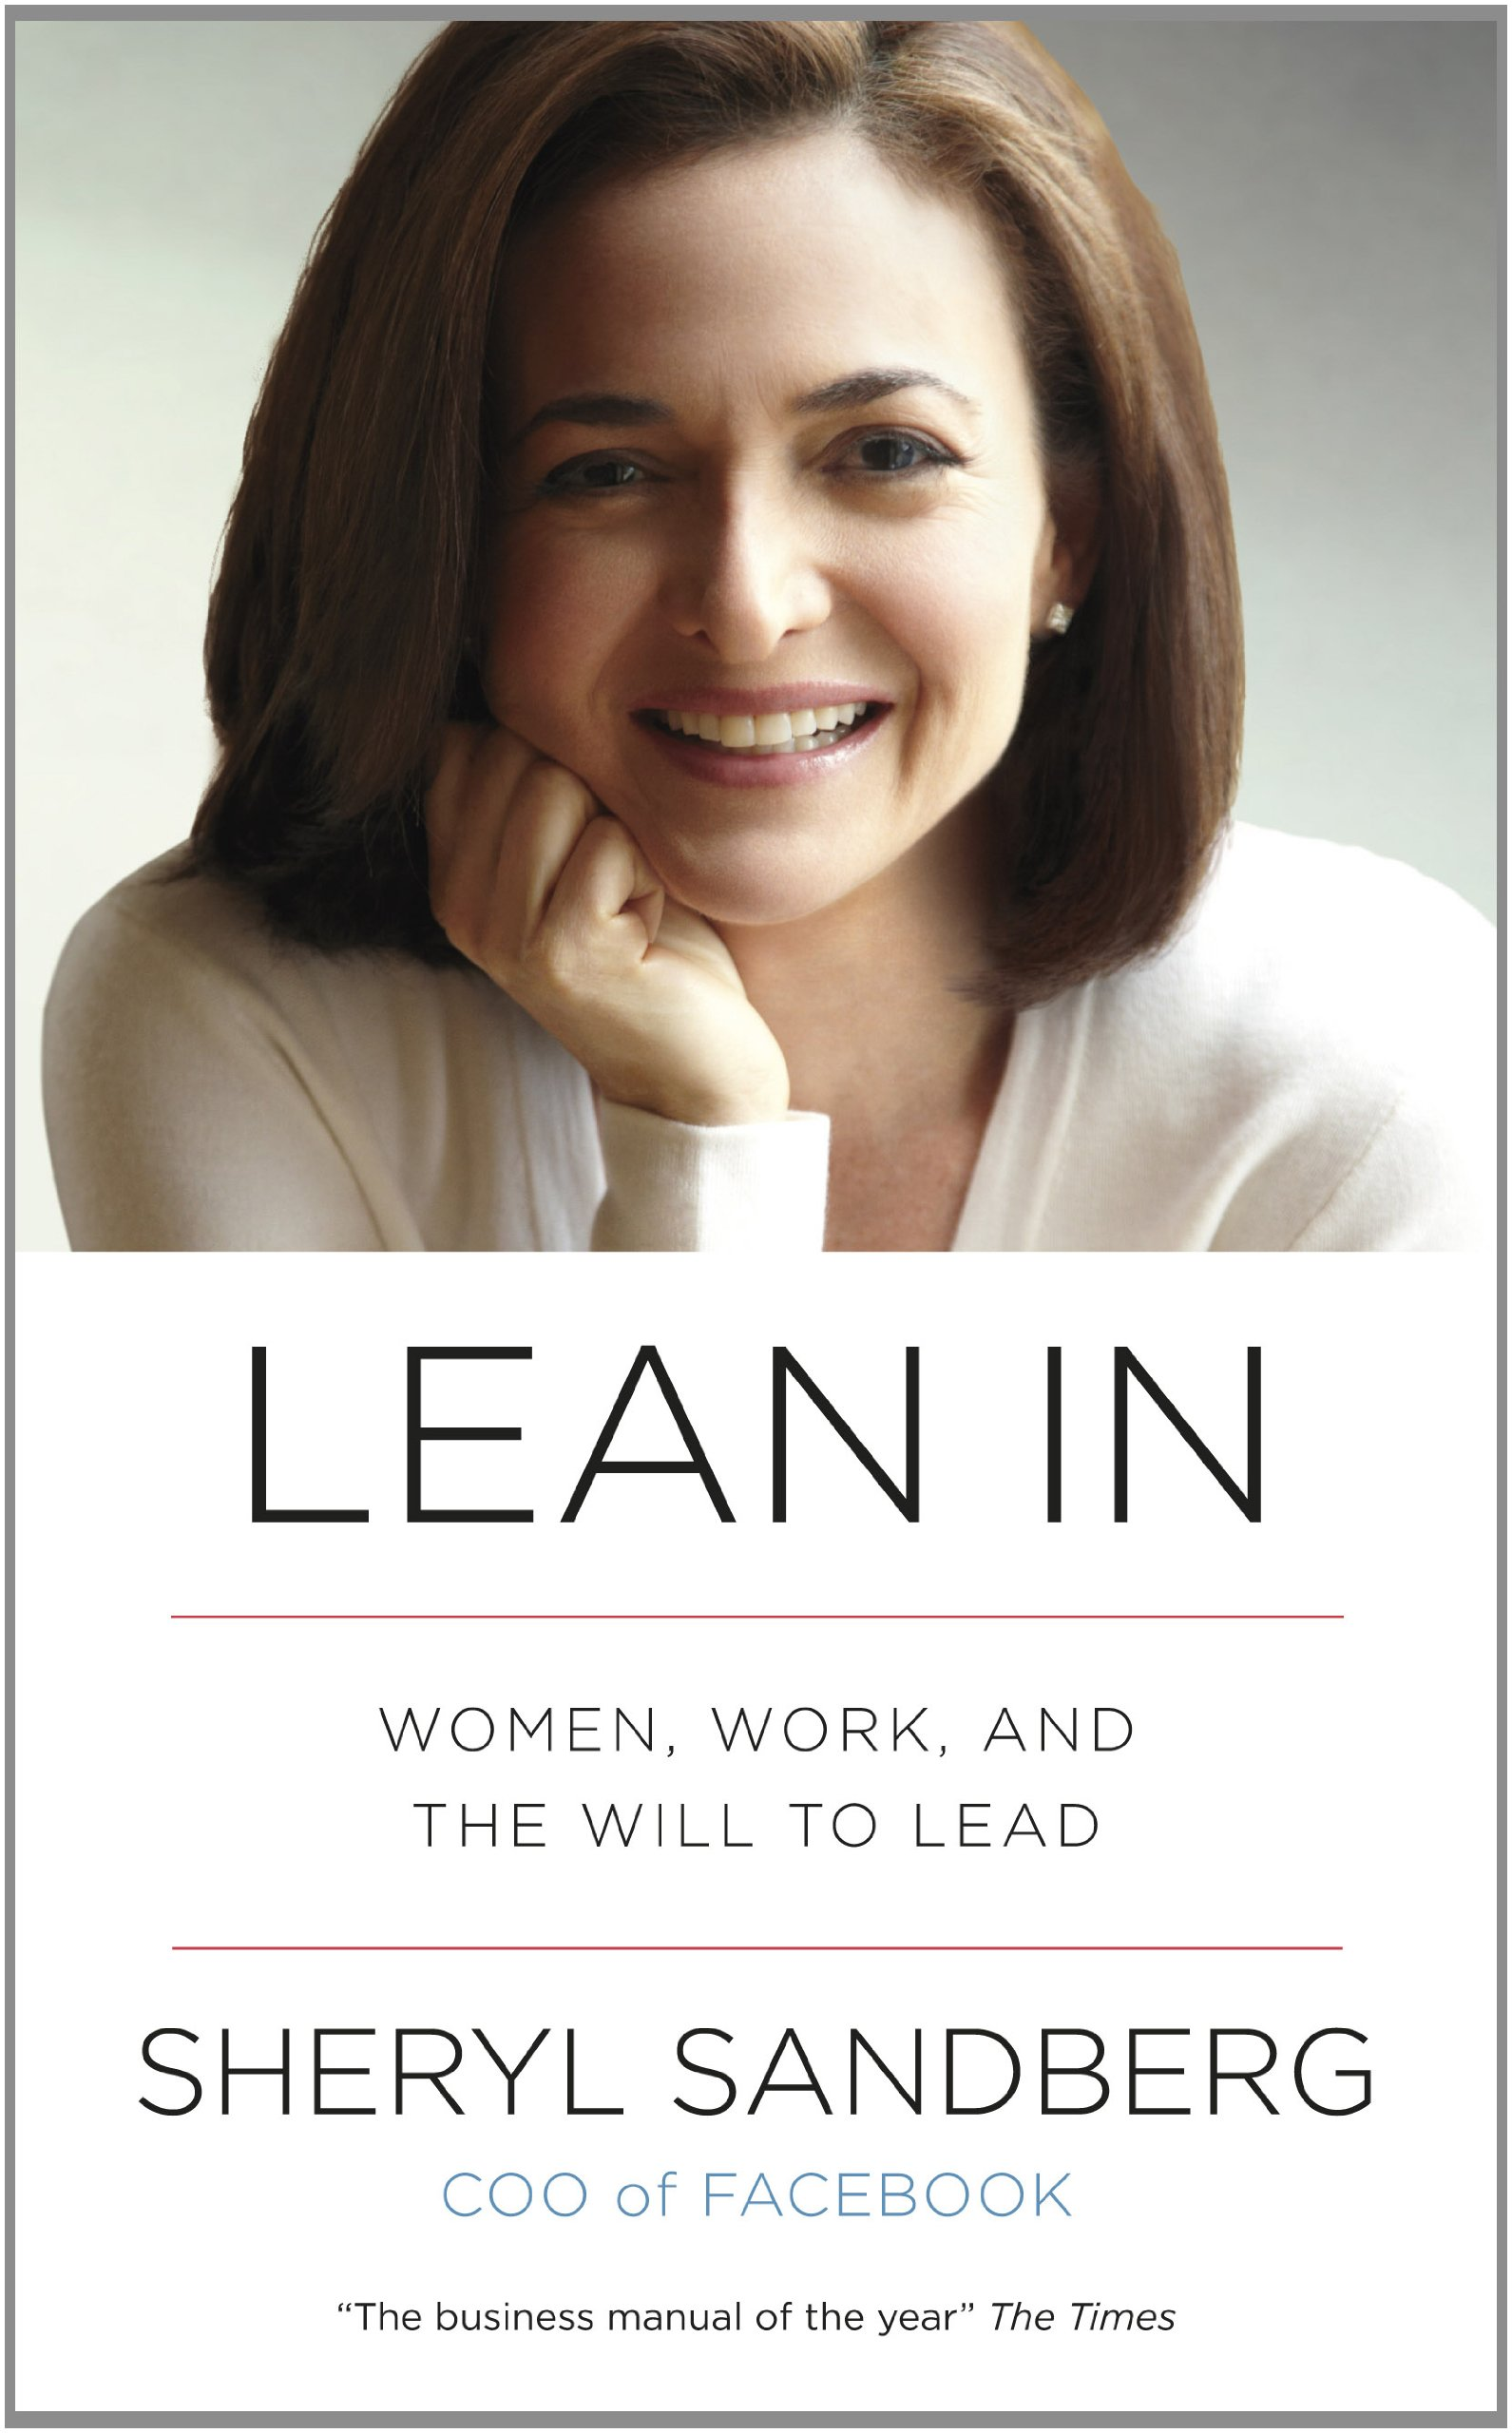
\includegraphics[width=4cm]{lean.jpg}
		\end{column}
		\begin{column}{0.5\textwidth}
			\begin{itemize}
					\pause
				\item Lean In
					\pause
				\item Lean Out
					\pause
				\item Lean sideways?
			\end{itemize}

		\end{column}
	\end{columns}
\end{frame}
\subsection{It's bad for tech}
\begin{frame}{we design better tech when we consider all the users. }

\end{frame}
\begin{frame}{The default male}
\end{frame}
\begin{frame}{Period trackers and menopause apps}
\end{frame}
\begin{frame}{Other examples}
\end{frame}
\begin{frame}{Technical imperative}
\end{frame}

\subsection{It's bad for women}
\begin{frame}{being in a minority isn't fun }

\end{frame}
\begin{frame}{Stereotype threat}
\end{frame}
\begin{frame}{Self efficacy}
\end{frame}
\begin{frame}{Sense of belonging }
\end{frame}
\begin{frame}{Macro and micro agressions}
\end{frame}
\begin{frame}{Petrie multiplier}
	\begin{columns}
		\begin{column}{0.5\textwidth}
			\animategraphics[loop,controls,width=4cm]{10}{petrie-}
		\end{column}
		\begin{column}{0.5\textwidth}
			\begin{itemize}
				\item Proposed by Karen Petrie, made popular by Ian Gent (who also made the gif).\footnote{Extensions of this have been proposed: \url{https://doi.org/10.1088/1751-8113/48/27/27FT01}}
					\pause
				\item Lean In
					\pause
				\item Lean Out
					\pause
				\item Lean sideways?
			\end{itemize}

		\end{column}
	\end{columns}
\end{frame}
\begin{frame}{Diversity tax}
\end{frame}

\begin{frame}{Moral imperative}
\end{frame}
\subsection{It's bad for men}

\begin{frame}{social}

\end{frame}

\begin{frame}{What's good for the goose is good for the gander}
	``A profession that's good for women is good for all'' - Rebecca George 

	\begin{itemize}
		\item Childcare
		\item Flexible working
	\end{itemize}
\end{frame}

\begin{frame}{Self-interest}

\end{frame}

\section{Don't do this}

\begin{frame}{Don't be that guy}

\end{frame}

\begin{frame}{Don't assume women are in sales}

\end{frame}
\begin{frame}{Don't talk over women}

\end{frame}
\begin{frame}{Don't pay women less}

\end{frame}

\section{Do do this}

\begin{frame}{Be an ally}

\end{frame}
\begin{frame}{The really easy stuff}
	\begin{itemize}
		\item Amplify women's voices
		\item Encourage women and girls : ``you can do this''
		\item Talk about your salary
	\end{itemize}
\end{frame}
\begin{frame}{Learn about the law}
	Discrimination first aider

\end{frame}

\begin{frame}{Consider workload}
	\begin{itemize}
		\item There's a workload associated with being in a minority
		\item \textbf{Diversity tax}
		\item Mentoring, panels, speaking, pastoral care
		\item Also: actual extra work 
		\item (This is ignoring the shadow workload of harassment tribunals, equal pay appeals, and discrimination cases)
	\end{itemize}
	If you're a manager, can you take this into account?  
\end{frame}

\begin{frame}{Volunteer}
        Pick up some of the diversity work. 
	\begin{itemize}
		\item Make sure the events you organise are safe for minorities
		\item Help organise events for minority groups
		\item Mentor and sponsor people from minority groups 
		\item Don't leave women to do the pastoral stuff 
	\end{itemize}
\end{frame}
\begin{frame}{Consider the cost of activities}
	\begin{itemize}
		\item Events after work or at weekends aren't accessible to all
		\item Refunding work travel after the fact can be problematic for those with financial constraints
	\item Travel can be hard for those with caring responsibilities
	\item Some countries can be dangerous for LGBT+ colleagues, or those from ethnic minorites
	\end{itemize}
\end{frame}

\begin{frame}{Consider homogenisation}
	\begin{itemize}
		\item Not every woman wants to get involved in diversity stuff.
		\item Not every asian colleague will be observing Ramadan right now. 
		\item Not every colleague observing Ramandan right now will be asian.  
	\end{itemize}
\end{frame}

\begin{frame}{Foster self-efficacy}
\end{frame}
\begin{frame}{Foster a sense of belonging}
\end{frame}

\begin{frame}{Consider intersectionality}
\end{frame}

\section{Conclusions}
	\begin{frame}{We all need to take diversity seriously}
		\begin{itemize}
		\item It's bad for tech, business, minorities and majorities 
		\item Women can't fix it on our own
		\begin{itemize}
			\item It's bad for us
			\item It's bad for our careers
			\item It's bad for tech
		\end{itemize}
	\end{itemize}
	\end{frame}
\begin{frame}{Any questions?}

	\begin{itemize}
	\item Questions?
	\item Thoughts?
	\item Disagreements?
	\end{itemize}
\end{frame}


\end{document}
